% D_Exp_2

The main aim of Experiment 2 was to see whether vagueness would exert beneficial effects when all conditions used numerals in the instructions, and when there were vague and crisp versions of the instructions for both comparison and matching strategies. The main changes from Experiment 1 were that the human selection task was explicitly controlled (i.e., whether the task amounted to matching or comparison), and that all conditions were constrained to mention a number. We used the same arrays as in Experiment 1 (an example stimulus is given in Figure \ref{Experiment1and2examplestimulus}). We used a 2 x 2 factorial manipulation of vagueness and selection task (see Table \ref{Instructions for e2}). On each trial an instruction was presented: participants pressed a key to dismiss the instruction, at which time the dot arrays were presented until the participant responded, and the response time and choice were recorded. Table \ref{Instructions for e2} shows the instructions for each condition. Note the difference between ``fewer than 20'' and ``far fewer than 20'': whereas the former cannot have borderline cases (i.e., for each number it is clear whether the number is smaller than 20 or not), the latter can.

\begin{table}
\centering
\caption{Experiment 2: Instructions arranged by condition. The instructions given in the table started with ``Choose a square with \ldots"} 
\label{Instructions for e2}
\begin{tabular}{cccll}
\hline\noalign{\smallskip}
Item & Quantity & Selection & Crisp & Vague \\ 
\noalign{\smallskip}\hline\noalign{\smallskip}
06:15:24 & Small & Comparison & fewer than 20 dots & far fewer than 20 dots \\ 
06:15:24 & Small & Matching & 6 dots & about 10 dots \\ 
06:15:24 & Large & Comparison & more than 10 dots & far more than 10 dots \\ 
06:15:24 & Large & Matching & 24 dots & about 20 dots \\ 
\noalign{\smallskip}\hline\noalign{\smallskip}
16:25:34 & Small & Comparison & fewer than 30 dots & far fewer than 30 dots \\ 
16:25:34 & Small & Matching & 16 dots & about 20 dots \\ 
16:25:34 & Large & Comparison & more than 20 dots & far more than 20 dots \\ 
16:25:34 & Large & Matching & 34 dots & about 30 dots \\ 
\noalign{\smallskip}\hline\noalign{\smallskip}
26:35:44 & Small & Comparison & fewer than 40 dots & far fewer than 40 dots \\ 
26:35:44 & Small & Matching & 26 dots & about 30 dots \\ 
26:35:44 & Large & Comparison & more than 30 dots & far more than 30 dots \\ 
26:35:44 & Large & Matching & 44 dots & about 40 dots \\ 
\noalign{\smallskip}\hline\noalign{\smallskip}
36:45:54 & Small & Comparison & fewer than 50 dots & far fewer than 50 dots \\ 
36:45:54 & Small & Matching & 36 dots & about 40 dots \\ 
36:45:54 & Large & Comparison & more than 40 dots & far more than 40 dots \\ 
36:45:54 & Large & Matching & 54 dots & about 50 dots \\ 
\noalign{\smallskip}\hline
\end{tabular}
\end{table}

\subsection{Hypotheses (Experiment 2)}

For Experiment 2, we formulated the following hypotheses:

\begin{description}
	\item [Hypothesis 1 (Crisp/Vague RT)] Vague instructions should result in faster responses than crisp instructions.
	\item [Hypothesis 2 (Comparison/Matching RT)] Instructions that allow comparison should result in faster responses than instructions that necessitate matching.
	\item [Hypothesis 3 (Interaction)] The vagueness effect should differ according to whether the selection task is comparison or matching.
\end{description}

\subsection{Results (Experiment 2)}

38 participants were recruited. Response times from all trials were trimmed at 2.5 standard deviations for each subject, leading to the loss of 204 trials (2.8\% of the trials). The distribution of remaining response times was skewed with many long responses. These remaining response times were log-transformed which reduced this skew so that their distribution more closely approximated a normal distribution. Condition means for response times are plotted in Figure \ref{resultsD-exp-2}. 

\begin{figure}[htbp]
\centering
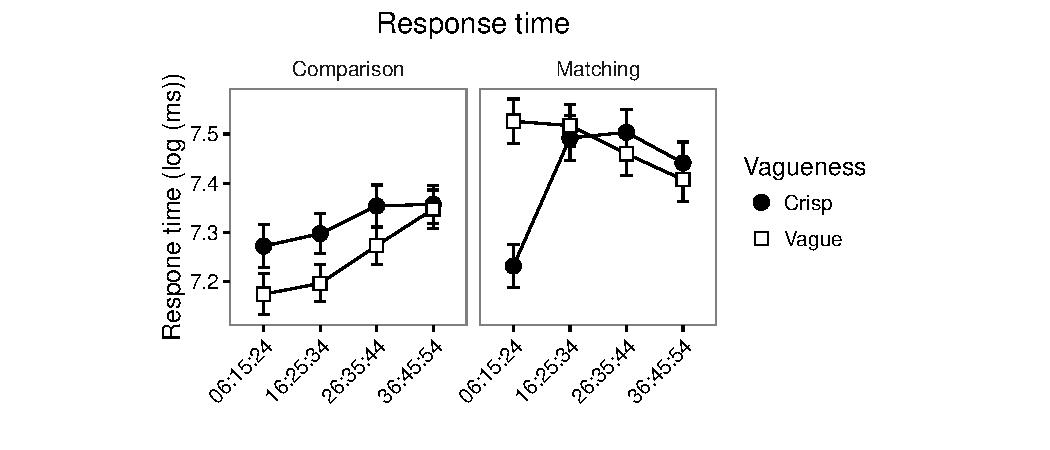
\includegraphics[width=\textwidth]{figures/De2-rtplot-1.pdf}
\caption{Mean response times by condition for Experiment 2 where all instructions were numeric}
\label{resultsD-exp-2}
\end{figure}

A linear mixed model was constructed for the logged response times, with sum-coded vagueness, selection task, and their interaction, and item as fixed effects, and per-participant intercepts and slopes for sum-coded vagueness, selection task, and their interaction, and item for random effects.

\begin{description} 
	\item [Test of Hypothesis 1 (Crisp/Vague RT)] Vague instructions resulted in faster responses than crisp instructions on average. However this difference was not significant in the full model ($\beta=-0.0057$, $se=0.0137$, $t=-0.42$, $p=0.678$). Using Levy's method \citep{Levy:MainEffectsInteractions} to test for main effects in the presence of higher-order interactions, by doing model comparison between a null model that included all interaction terms involving Vagueness but leaving out a term for the main effect of Vagueness, against a full model that differed only by including Vagueness as a main effect, showed that the full model was no better than the reduced model ($df=1$, $p=0.676$), consituting more evidence that Vagueness did not exert a significant main effect on response times. 
	\item [Test of Hypothesis 2 (Comparison/Matching RT)] Instructions involving comparison resulted in faster responses than instructions involving matching, and the difference was significant ($\beta=0.1618$, $se=0.0255$, $t=6.34$, $p<0.001$).
	\item [Test of Hypothesis 3 (Interaction)] The interaction between Vagueness and Selection task was significant ($\beta=0.1306$, $se=0.0205$, $t=6.38$, $p<0.001$), showing that vagueness exerted different effects on response times according to whether the instructions involved comparison or matching. When separate analyses were carried out testing for the effect of vagueness in comparison-only and in matching-only conditions, vague instructions led to significantly \emph{faster} responses than crisp instructions in the comparison-only conditions ($\beta=-0.071$, $se=0.020$, $t=-3.52$, $p<0.01$); and in the matching-only conditions vague instructions led to significantly \emph{slower} responses than crisp instructions ($\beta=0.062$, $se=0.021$, $t=2.91$, $p<0.01$).
\end{description}

\subsection{Discussion (Experiment 2)}

The cost reduction account predicted that there should be a significant main effect of Vagueness such that responses would be faster for Vague intructions than for crisp instructions. We found that although there was a very small effect in that direction, the effect was not statistically significant. Models that differed only in the presence of Vagueness as a main effect were shown not to differ significantly in their explanatory value. However we did find that Vagueness exerted effects on other variables: Vagueness speeded RTs in the comparison task and slowed RTs in the matching task.
